\snote{brun}

\subsection*{Motivation}

This note examines whether a simpler, purely sensitivity-based selection criterion achieves an external validation accuracy comparable to that of our method, which additionally tests admissibility and applies backward elimination. We compared against column-pivoted QR selection (Vélez-Reyes and Verghese, 1995), a well-established subset-selection method that selects parameters by their linear independence in the sensitivity matrix, without re-estimation or test-set evaluation. The collinearity index of Brun \emph{et al.} (Brun et al., 2001) is a different criterion and is compared separately in \sref{morrisbrun}.

\subsection*{Method: QR-pivoted selection}

\paragraph{Sensitivity matrix.}
For each problem the normalised sensitivity matrix $\widetilde{J}\in\mathbb{R}^{n_{\mathrm{obs}}\times n_{\mathrm{bio}}}$ is computed at $\theta_0$ on the training data using forward finite differences.  Column $j$ is
\[
  \widetilde{J}_{\cdot j} = \frac{\partial z / \partial\theta_j}{\|\partial z / \partial\theta_j\|_2},
  \qquad
  \frac{\partial z_i}{\partial\theta_j} \approx \frac{z_i(\theta_0 + \varepsilon_j e_j) - z_i(\theta_0)}{\varepsilon_j},
\]
where $\varepsilon_j = \max(10^{-4}|\theta_{0,j}|,\, 10^{-8})$ and $n_{\mathrm{obs}}$ counts training-data points with finite measurements. Columns with $\|\partial z/\partial\theta_j\|_2 \le 10^{-10}$ (zero sensitivity) are discarded before pivoting.

\paragraph{Column-pivoted QR.}
Pivoted QR decomposition of $\widetilde{J}$ is
\[
  \widetilde{J}\,P = Q\,R, \qquad |R_{11}| \ge |R_{22}| \ge \cdots,
\]
where $P$ is a column-permutation matrix.  The leading pivot columns of $\widetilde{J}\,P$---equivalently, the first entries of $P$---correspond to the parameters that contribute most independently to the measured outputs.

\paragraph{Subset selection.}
For each problem we select the top $k = |S|$ biological parameters from the QR ranking and append the same calibration parameters $\Theta_C$ used in the original analysis.

\paragraph{Validation.}
The QR-selected subset is fitted on the training data using the same optimiser (trust-region reflective least squares) and the same number of function evaluations as the original reduced model.  Test-set $\chi^2/n$ is then computed identically to the main experiment.  The test set is never consulted at any stage of the QR selection or fitting.

\subsection*{Results}

Figure~\ref{fig:brun_scatter} compares $\chi^2_{\mathrm{ours}}$ and $\chi^2_{\mathrm{QR}}$ for all 28 evaluated problems.  The grey band marks $\pm$5\% equivalence.  Points on or near the diagonal correspond to problems where both methods achieve essentially the same predictive accuracy despite---in most cases---choosing entirely different parameters.

Among 26 non-trivial comparisons (both $\chi^2 > 10^{-3}$) the median ratio $\chi^2_{\mathrm{QR}}/\chi^2_{\mathrm{ours}} = 0.99$ and 15 problems fall within the $\pm$5\% band.  QR predicted better by more than 5\% in 9 problems (most notably Boehm and Brannmark) and our method predicted better in 2 (most notably Oliveira, where $\chi^2_{\mathrm{QR}} = 80\times\chi^2_{\mathrm{ours}}$; the QR-selected parameters failed to capture the epidemic dynamics on the test partition).  In two additional problems (Giordano, Perelson) both methods fit the test data to within machine precision, making the ratio uninformative.

The most striking result is that the two methods selected \emph{completely different} biological parameters in 19 of 28 problems (Table~\ref{tab:brun_params}); the median overlap was 0 shared parameters.  In 9 problems they shared exactly one parameter; in one problem (Perelson) they agreed completely.  Despite this divergence, 22 of 26 comparisons produced ratios between 0.5 and 2.0.  This is consistent with the sloppy-model picture (Gutenkunst et al., 2007): many distinct parameter combinations describe the training data approximately equally well, so the test-set $\chi^2/n$ is relatively insensitive to which specific $k$-parameter subset is selected.

The comparable performance of the two methods shows that the additional computational cost of the admissibility test and backward elimination does not translate into a systematic improvement in external validation accuracy on this benchmark.  Conversely, it also does not lead to a systematic loss of accuracy: the two dramatic failures of QR on Oliveira and the large improvements of QR on Boehm and Brannmark are problem-specific and cancel on aggregate.  Our method's value relative to pivoted-QR selection lies in the admissibility test (the reduced model is verified numerically to reproduce the full model's outputs under parameter perturbations; \sref{admisother} shows that pivoted-QR subsets pass this test in only 13 of 29 problems) and in the systematic backward elimination that delivers a minimal subset, not in a predictive accuracy advantage.

\begin{figure}[H]
\centering
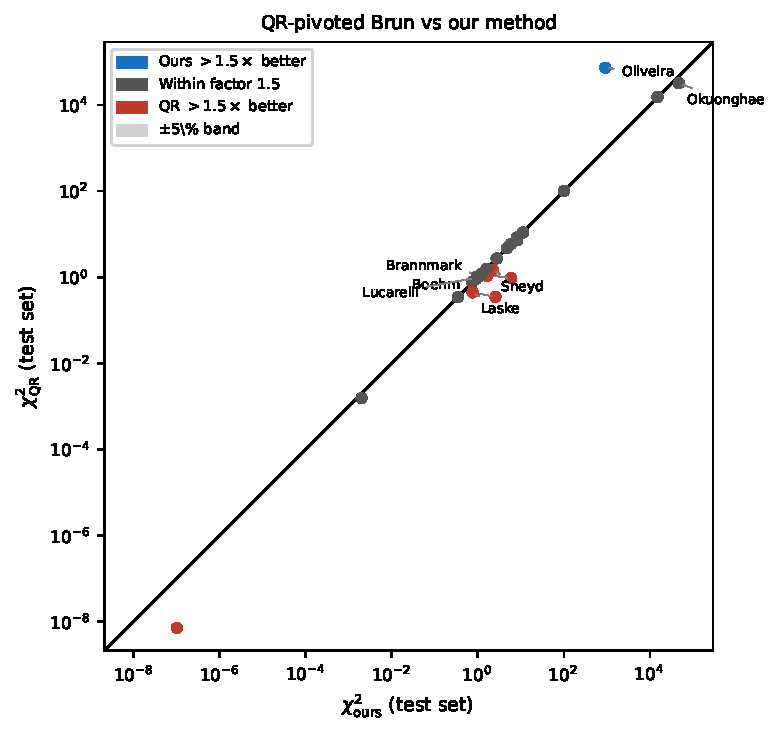
\includegraphics[width=0.58\textwidth]{figures/fig_brun.pdf}
\caption{Scatter plot of test-set $\chi^2/n$ for our method ($x$-axis) versus pivoted-QR selection ($y$-axis), on a log-log scale.  Each point is one of the 28 evaluated problems; two with $\chi^2 < 10^{-13}$ (Perelson, Giordano) lie below the plot range and are omitted.  The solid diagonal is the 1:1 line; the grey band marks $\pm$5\%.  Blue: ours more than $1.5\times$ better; red: QR more than $1.5\times$ better; grey: within factor 1.5.  Notable problems are labelled.}
\label{fig:brun_scatter}
\end{figure}

\subsection*{Selected parameters}

Table~\ref{tab:brun_params} lists the biological parameters selected by each method for every problem.  Parameter names follow the model's own PEtab identifiers.  The overlap column gives the number of shared selections.

{\scriptsize
\begin{longtable}{@{}>{\raggedright\arraybackslash}p{2.3cm}r>{\raggedright\arraybackslash}p{4.0cm}>{\raggedright\arraybackslash}p{4.0cm}c@{}}
\caption{Biological parameters selected by our method ($S_{\mathrm{ours}}$) and by column-pivoted QR ($S_{\mathrm{QR}}$) for each evaluated problem. \emph{Overlap}: number of parameters shared by both subsets. Parameter names are PEtab identifiers; long names are line-broken.}\label{tab:brun_params}\\
\toprule
Problem & $k$ & $S_{\mathrm{ours}}$ & $S_{\mathrm{QR}}$ & Ovlp \\
\midrule \endfirsthead
\toprule Problem & $k$ & $S_{\mathrm{ours}}$ & $S_{\mathrm{QR}}$ & Ovlp \\ \midrule \endhead
Alkan & 2
  & \texttt{kt}, \texttt{k\_\allowbreak{}rep\_\allowbreak{}nhej}
  & \texttt{p\_\allowbreak{}chk1\_\allowbreak{}dea\_\allowbreak{}wip1}, \texttt{k\_\allowbreak{}death\_\allowbreak{}reox}
  & 0 \\
Armistead & 2
  & \texttt{k\_\allowbreak{}d}, \texttt{alpha\_\allowbreak{}cer}
  & \texttt{k00}, \texttt{k2}
  & 0 \\
Bachmann & 2
  & \texttt{CISRNADelay}, \texttt{JAK2ActEpo}
  & \texttt{SOCS3Inh}, \texttt{CISEqcOE}
  & 0 \\
Boehm & 2
  & \texttt{k\_\allowbreak{}imp\_\allowbreak{}hetero}, \texttt{k\_\allowbreak{}phos}
  & \texttt{k\_\allowbreak{}phos}, \texttt{k\_\allowbreak{}imp\_\allowbreak{}homo}
  & 1 \\
Borghans & 2
  & \texttt{Kz}, \texttt{K\_\allowbreak{}par}
  & \texttt{Kd}, \texttt{init\_\allowbreak{}A\_\allowbreak{}state}
  & 0 \\
Brannmark & 2
  & \texttt{k1f}, \texttt{km2}
  & \texttt{k1a}, \texttt{k\_\allowbreak{}IRSiP\_\allowbreak{}DosR}
  & 0 \\
Bruno & 5
  & \texttt{kb1}, \texttt{init\_\allowbreak{}bcar2}, \texttt{init\_\allowbreak{}zea\_\allowbreak{}1}, \texttt{init\_\allowbreak{}bcar1}, \texttt{init\_\allowbreak{}bcry\_\allowbreak{}1}
  & \texttt{init\_\allowbreak{}b10\_\allowbreak{}1}, \texttt{init\_\allowbreak{}bcar1}, \texttt{kc4}, \texttt{kc1}, \texttt{kc2}
  & 1 \\
Elowitz & 2
  & \texttt{n\_\allowbreak{}Hill}, \texttt{tau\_\allowbreak{}mRNA}
  & \texttt{eff\_\allowbreak{}GFP}, \texttt{tau\_\allowbreak{}prot\_\allowbreak{}GFP}
  & 0 \\
Fiedler & 2
  & \texttt{tau2}, \texttt{k6}
  & \texttt{k11}, \texttt{k5}
  & 0 \\
Fujita & 2
  & \texttt{init\_\allowbreak{}AKT}, \texttt{reaction\_\allowbreak{}6\_\allowbreak{}k1}
  & \texttt{reaction\_\allowbreak{}1\_\allowbreak{}k1}, \texttt{reaction\_\allowbreak{}6\_\allowbreak{}k1}
  & 1 \\
Giordano & 2
  & \texttt{alpha\_\allowbreak{}4}, \texttt{alpha\_\allowbreak{}28}
  & \texttt{delta\_\allowbreak{}0}, \texttt{eta\_\allowbreak{}0}
  & 0 \\
Isensee & 2
  & \texttt{kf\_\allowbreak{}RIIp\_\allowbreak{}C\_\allowbreak{}2\_\allowbreak{}\_\allowbreak{}RII\_\allowbreak{}C\_\allowbreak{}2}, \texttt{xi\_\allowbreak{}kf\_\allowbreak{}RII\_\allowbreak{}C\_\allowbreak{}2\_\allowbreak{}\_\allowbreak{}RII\_\allowbreak{}2}
  & \texttt{kf\_\allowbreak{}Fsk}, \texttt{KD\_\allowbreak{}H89}
  & 0 \\
Laske & 2
  & \texttt{k\_\allowbreak{}imp}, \texttt{k\_\allowbreak{}syn\_\allowbreak{}R\_\allowbreak{}M}
  & \texttt{k\_\allowbreak{}imp}, \texttt{k\_\allowbreak{}rel}
  & 1 \\
Liu & 2
  & \texttt{kappa}, \texttt{phi}
  & \texttt{kappa}, \texttt{rho}
  & 1 \\
Lucarelli & 10
  & \texttt{init\_\allowbreak{}Rec}, \texttt{S2tot}, \texttt{S3tot}, \texttt{S\_\allowbreak{}dephosphos}, \texttt{S\_\allowbreak{}phos}, \texttt{geneF\_\allowbreak{}turn}, \texttt{k\_\allowbreak{}234}, \texttt{geneK\_\allowbreak{}turn}, \texttt{S4tot}, \texttt{geneH\_\allowbreak{}turn}
  & \texttt{S4tot}, \texttt{geneK\_\allowbreak{}turn}, \texttt{geneJ\_\allowbreak{}turn}, \texttt{geneB\_\allowbreak{}act2}, \texttt{geneG\_\allowbreak{}act1}, \texttt{geneH\_\allowbreak{}turn}, \texttt{geneL\_\allowbreak{}turn}, \texttt{geneE\_\allowbreak{}act2}, \texttt{geneI\_\allowbreak{}act1}, \texttt{geneC\_\allowbreak{}act1}
  & 3 \\
Okuonghae & 2
  & \texttt{transmission\_\allowbreak{}rate\_\allowbreak{}effective}, \texttt{gamma\_\allowbreak{}i}
  & \texttt{asymptomatic\_\allowbreak{}start}, \texttt{d\_\allowbreak{}D}
  & 0 \\
Oliveira & 2
  & \texttt{beta\_\allowbreak{}0}, \texttt{h\_\allowbreak{}hosp\_\allowbreak{}rate}
  & \texttt{beta\_\allowbreak{}1}, \texttt{symptomatic\_\allowbreak{}init\_\allowbreak{}concentration}
  & 0 \\
Perelson & 2
  & \texttt{c}, \texttt{delta}
  & \texttt{c}, \texttt{delta}
  & 2 \\
Rahman & 2
  & \texttt{infected\_\allowbreak{}moderate\_\allowbreak{}transmission\_\allowbreak{}rate}, \texttt{infected\_\allowbreak{}normal\_\allowbreak{}worsen\_\allowbreak{}rate}
  & \texttt{infected\_\allowbreak{}moderate\_\allowbreak{}transmission\_\allowbreak{}rate}, \texttt{treated\_\allowbreak{}moderate\_\allowbreak{}improve\_\allowbreak{}rate}
  & 1 \\
Raia & 2
  & \texttt{SOCS3mRNA\_\allowbreak{}production}, \texttt{init\_\allowbreak{}Rec\_\allowbreak{}i}
  & \texttt{Rec\_\allowbreak{}recycle}, \texttt{DecoyR\_\allowbreak{}binding}
  & 0 \\
Raimundez & 2
  & \texttt{kdeg\_\allowbreak{}membran\_\allowbreak{}\_\allowbreak{}MKN1}, \texttt{d\_\allowbreak{}kimp\_\allowbreak{}pEGFR\_\allowbreak{}EGF\_\allowbreak{}2\_\allowbreak{}\_\allowbreak{}MKN1\_\allowbreak{}2\_\allowbreak{}HS746T}
  & \texttt{d\_\allowbreak{}MAPKtotal\_\allowbreak{}\_\allowbreak{}MKN1\_\allowbreak{}2\_\allowbreak{}HS746T}, \texttt{d\_\allowbreak{}MPI3Ktotal\_\allowbreak{}\_\allowbreak{}fm\_\allowbreak{}2\_\allowbreak{}hm}
  & 0 \\
Salazar-Cavazos & 2
  & \texttt{ratio\_\allowbreak{}kpkd\_\allowbreak{}Y1068\_\allowbreak{}\_\allowbreak{}FREE}, \texttt{ratio\_\allowbreak{}kpkd\_\allowbreak{}YN\_\allowbreak{}\_\allowbreak{}FREE}
  & \texttt{GRB2\_\allowbreak{}total\_\allowbreak{}\_\allowbreak{}FREE}, \texttt{kdephosYN\_\allowbreak{}\_\allowbreak{}FREE}
  & 0 \\
Schwen & 2
  & \texttt{ini\_\allowbreak{}R1}, \texttt{ini\_\allowbreak{}R2fold}
  & \texttt{kd2fold}, \texttt{kout}
  & 0 \\
Smith & 2
  & \texttt{k8}, \texttt{kminus7b}
  & \texttt{kminus7a}, \texttt{k43r}
  & 0 \\
Sneyd & 2
  & \texttt{l4}, \texttt{l2}
  & \texttt{k\_\allowbreak{}2}, \texttt{k\_\allowbreak{}3}
  & 0 \\
Weber & 2
  & \texttt{s12}, \texttt{a21}
  & \texttt{a22}, \texttt{pu5}
  & 0 \\
Zhao & 3
  & \texttt{R\_\allowbreak{}Stage\_\allowbreak{}I\_\allowbreak{}China}, \texttt{R\_\allowbreak{}Stage\_\allowbreak{}II\_\allowbreak{}Wuhan}, \texttt{gamma\_\allowbreak{}1\_\allowbreak{}Stage\_\allowbreak{}I\_\allowbreak{}Hubei}
  & \texttt{R\_\allowbreak{}Stage\_\allowbreak{}I\_\allowbreak{}Wuhan}, \texttt{R\_\allowbreak{}Stage\_\allowbreak{}III\_\allowbreak{}Wuhan}, \texttt{R\_\allowbreak{}Stage\_\allowbreak{}II\_\allowbreak{}Hubei}
  & 0 \\
Zheng & 2
  & \texttt{k01\_\allowbreak{}02}, \texttt{k13\_\allowbreak{}12}
  & \texttt{k01\_\allowbreak{}11}, \texttt{k10\_\allowbreak{}00}
  & 0 \\
\bottomrule
\end{longtable}}
